\documentclass[notitlepage]{report}

\author{Cronqvist, Fredrik \and Larsson, Sebastian \and Stenberg, Victor \and S\"{a}ll, Martin}
\date{\today}
\title{League of Legends learning analysis}

\usepackage{graphicx}

\begin{document}
\maketitle

\begin{abstract}
[Placeholder text]
\end{abstract}

\begingroup
\chapter*{Preface}
We would like to thank Emelie and Pontysius the Great for participating in our experiment.

\let\clearpage\relax

\tableofcontents
\endgroup

\chapter{Introduction}
This report takes on some questions about where players playing the computer game League of Legends with different levels of experience focus on the screen, what their priorities are during gameplay and how long they take to finish a round in the game. In hopes of discovering a trend six participants have been eye-tracked while playing one round in the game. The participants will be referred to P1, P2, … and P6, in order of experience with the game, where P1 has the least experience and P6 has the most.

\section{League of Legends}
League of Legends (LoL) is a multiplayer online battle arena (moba) game. By default two teams of five players each, participate with the goal of destroying the base of the opposing team. Each player controls a hero with unique abilities on the battlefield trying to achieve this goal.

The map is split into three different `lanes' where most of the combat occurs, separated by a `jungle', a traversable area with less visibility and many twists and turns. Because of this layout, keeping track of the players on one's own team as well as opponents is important to successful tactics. This is primarily accomplished through the use of a mini-map, a small area in the lower right corner showing a top down view of the area with icons for each players, colored by team.

As the game progresses, each player accumulates gold, the in-game currency, which is meant to be spent in a shop located in each team's base to buy items that improves the player's stats for the duration of the game.

\section{Hypothesis and questions}
We believe there is a distinct difference between how new players and experienced players look at the screen to attain information. To find out if this is right and to find possible improvements, we have stated the following questions:

\begin{itemize}
\item Do the new players find the shop?
\item Do new players spend less time on the mini-map than experienced players?
\end{itemize}

\chapter{Analysis}
All of the data retrieved from the experiment are visualized using gaze plots and heat maps, and one of each has been generated for each participant in order to find differences. Participants were selected from two different groups in order to make a comparison. Group 1 (P1, P2 and P3) contains players with little to none experience with the game and group 2 (P4, P5, and P6) contains players with plenty of experience. For the group analysis each group has its group members' gaze plots and heat maps combined into a single gaze plot and a single heat map to help with the analysis.

\section{Group 1 analysis}
P1 and P2 have no experience with moba games and P3 has played about 10 hours. As for this group's heat map (Figure~\ref{heat_noob}) some data can be extracted. They have a great focus on the middle of the screen where their characters are and some focus on the skills in the middle bottom of the screen. They also spend much more time on the mini-map down to the right. Some of the places they don't look as much on are down to the left, on the character stats, items and how much gold they have. Also there was nearly no focus on the info on the other teammates and the game stats.

When it comes to the gaze plot, see Figure~\ref{gaze_noob}, some patterns can be found, mostly that they look nearly everywhere. Some places are more attractive than others and a pattern also found are that they go to the mini-map and then back again.

\begin{figure}[!ht]
\begin{minipage}[b]{0.45\linewidth}
\centering
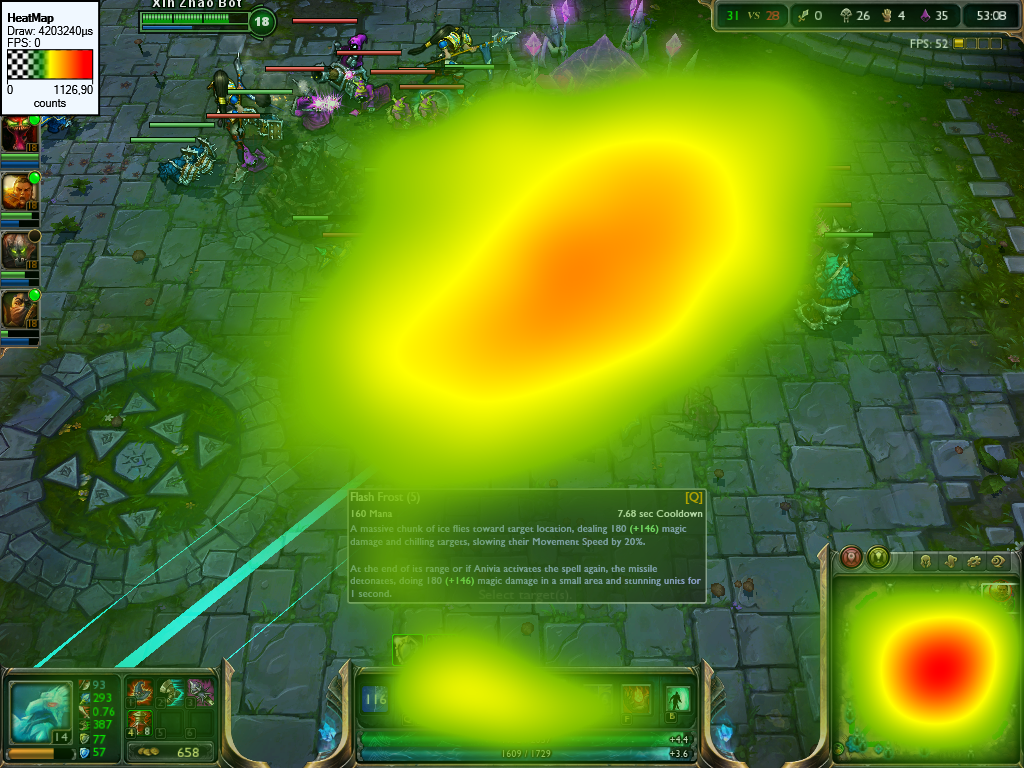
\includegraphics[width=\textwidth]{images/heatmap/Noobs}
\caption{Heat map Group 1}
\label{heat_noob}
\end{minipage}
\hspace{0.5cm}
\begin{minipage}[b]{0.45\linewidth}
\centering
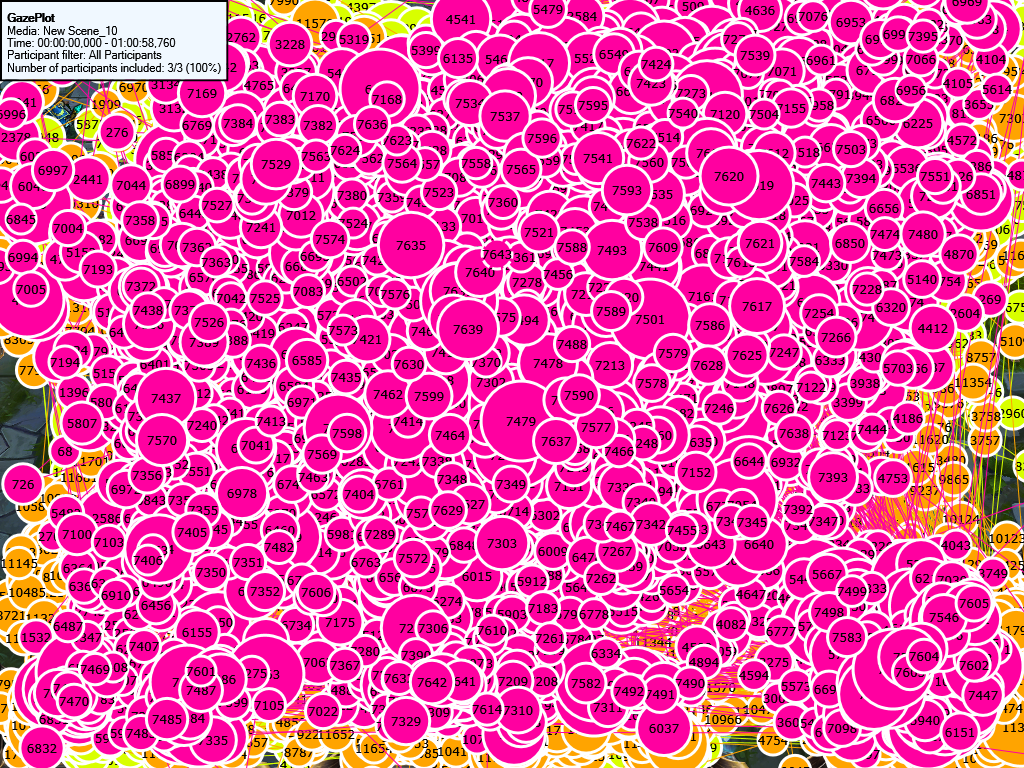
\includegraphics[width=\textwidth]{images/gazeplot/Noobs}
\caption{Gaze plot Group 1}
\label{gaze_noob}
\end{minipage}
\end{figure}

\section{Group 2 analysis}
P4, P5 and P6 have more than a years worth of experience with this type of games. This group's heat map, as seen in Figure~\ref{heat_pro}, have two main focus spots, one in the center of the screen and one on the first four skills in the bottom center. Some time are also spent on the mini-map and on the currently bought items.

As for the gaze plot in Figure~\ref{gaze_pro}, experienced players focus on the important information and focus less on the things around it. Often the time they spend looking for different information is very low except for on the center of the screen where the focus is on the battlefield.

\begin{figure}[!ht]
\begin{minipage}[b]{0.45\linewidth}
\centering
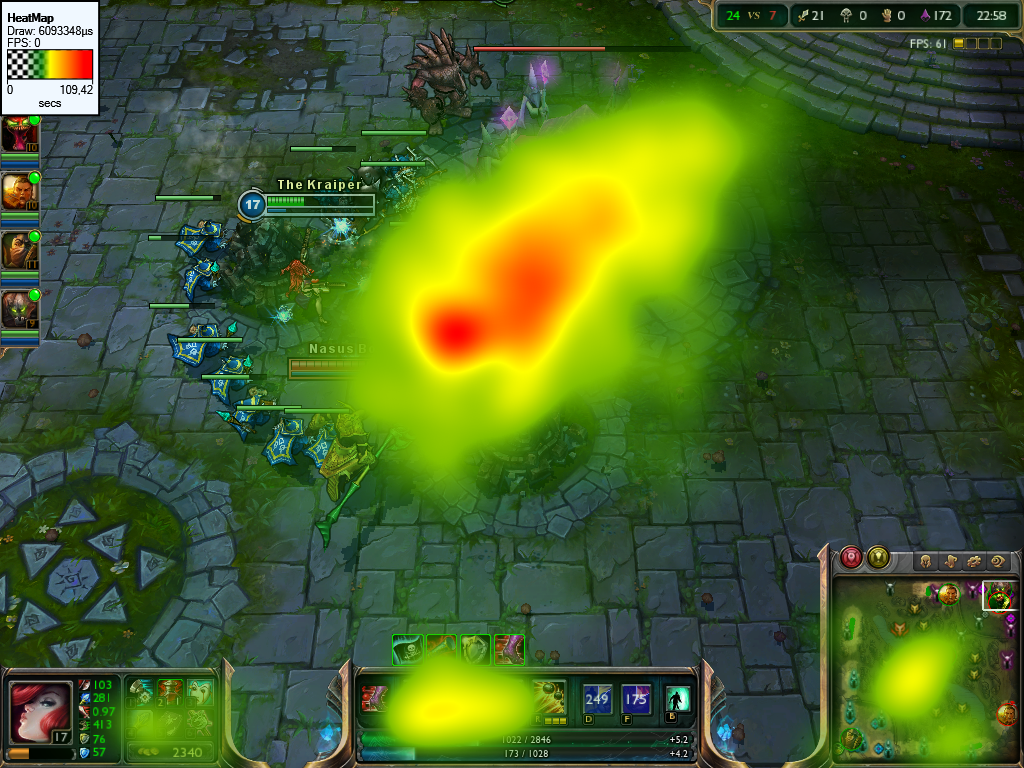
\includegraphics[width=\textwidth]{images/heatmap/Pros}
\caption{Heat map Group 2}
\label{heat_pro}
\end{minipage}
\hspace{0.5cm}
\begin{minipage}[b]{0.45\linewidth}
\centering
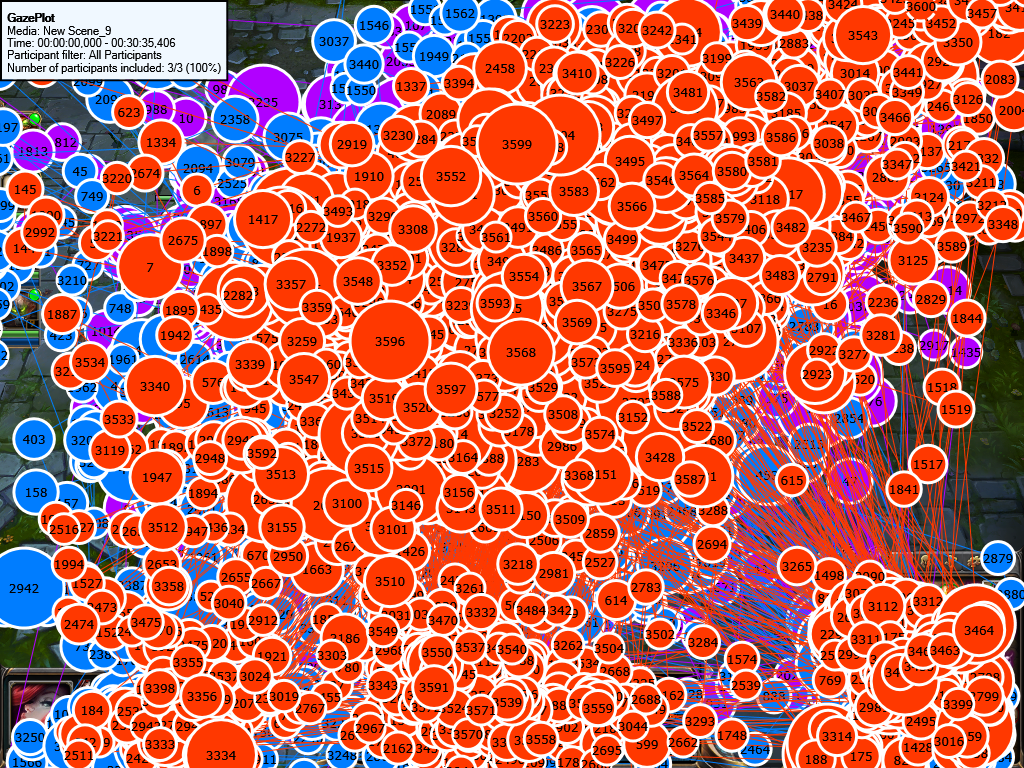
\includegraphics[width=\textwidth]{images/gazeplot/Pros}
\caption{Gaze plot Group 2}
\label{gaze_pro}
\end{minipage}
\end{figure}

\section{Discussion}
From a comparison between the gaze plots for the two groups, we can see that the experienced players keep their focus on the center of the screen and just quickly scan the abilities and the mini-map. This is also supported by the calculated focus percentage, as shown in Figure~\ref{aoi}. This is presumably to not miss any of the enemy champions actions.

\begin{figure}[h]
\centering
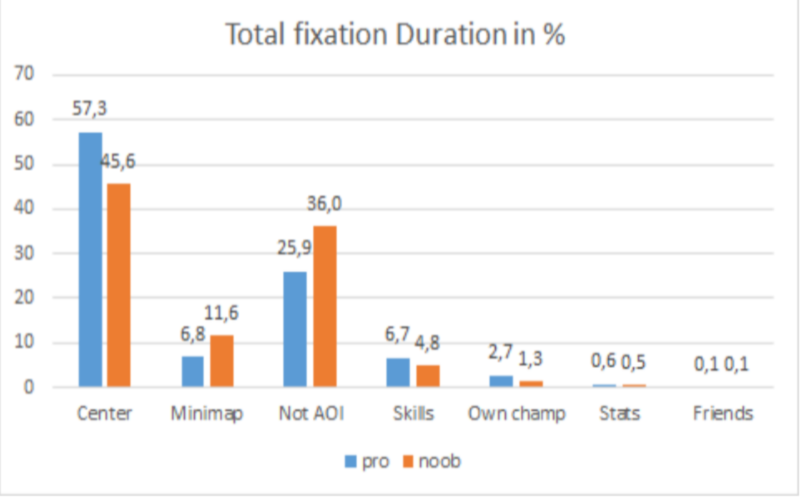
\includegraphics[width=0.8\textwidth]{images/AOIChart}
\caption{Graph showing the difference between how the two groups focus on areas of interest.}
\label{aoi}
\end{figure}

In comparison with this the less experienced players spend longer times on the mini-map and abilities per fixation and the focus on the center is spread in a much more uneven pattern from which it can be concluded that they don't know exactly what is the most important thing to focus on and instead try to see everything at the same time making it harder to make decisions.

From the heat maps the same trend can be seen but also that the experienced players spend quite a lot of time on the abilities, focused on the champions abilities and ignoring the summoner abilities. Some time is spent looking at the mini-map but the time spent looking there is significantly less than the time spent on the abilities or the center of the screen.

The less experienced players spend a lot of time on the mini-map and some in the center of the screen, but less on the abilities, see Figure~\ref{aoi}. The experienced players spend more time in the center of the screen and abilities but less on the mini-map. This suggests that the experienced players consider the action in the center of the screen and the abilities to be more important than the inexperienced do. The experience players also focus less on the edges of the screen and so the things that are happening close to the own champion have the main focus and the rest of the map is secondary.

\section{Conclusion}
The trend that can be read from this is that experienced players can faster read the information from the GUI elements and then focus back at the action around the center of the screen. This make it possible for those players to look at more places in the same time frame and then get more vital information to make more accurate and deadly decisions.

The experienced players spend more time focusing on the abilities, despite the fact that the inexperienced players spend extra time on reading the descriptions on the abilities, as they are not accustomed to them. This difference in focus is most likely because the experienced players consider the cooldown of abilities to be one of the most important GUI elements.

The question ``Do new players find the shop?'' was answered by questioning the participants and reviewing the replays. Of the inexperienced players P2 was the only one who never found the shop. P1 stumbled upon the shop after about 40 minutes of playing and P3 already knew about the shop from playing the tutorial. This suggests that without playing the tutorial a new player will have a hard time finding the shop without the influence from other players or other information.

Another question asked was, ``Do new players spend less time on the mini-map than experienced players?''. From the heat maps, gaze plots and the replays, a trend could be found where new players look less often at the mini-map but each time for a longer time, resulting in a larger total time. From this, it can be assumed that experienced players are more efficient in finding relevant information from the mini-map and have learned to quickly determine if they need to focus longer on the mini-map.

\end{document}
